\documentclass{article}

\usepackage[main, final]{neurips_2026}
\usepackage[utf8]{inputenc}
\usepackage[T1]{fontenc}
\usepackage{hyperref}
\usepackage{url}
\usepackage{booktabs}
\usepackage{amsfonts}
\usepackage{amsmath}
\usepackage{nicefrac}
\usepackage{microtype}
\usepackage{xcolor}
\usepackage{graphicx}
\usepackage{multirow}
\usepackage{array}
\usepackage{float}

\hypersetup{hidelinks}

\graphicspath{{../figures/}}

\title{Training Uzi: PPO for Lane-Dominant 1v1 Honor of Kings Agents}

\author{%
  Team Uzi\\
  Course Mini Paper Submission\\
  \texttt{repo: kaiwu}\\
}

\begin{document}

\maketitle

\begin{abstract}
We describe the training of \emph{Uzi}, a 1v1 Honor of Kings reinforcement-learning agent designed to play like an aggressive lane specialist. The name is an allusion to the League of Legends professional player Uzi: the design target was not passive survival, but pressure, spacing, target selection, and conversion from lane advantage into tower damage. Starting from the Kaiwu PPO baseline, we rebuilt the observation pipeline around structured entity tokens, added a hybrid MLP-token-LSTM policy, aligned the target head with environment target slots, repaired action legality for invalid attacks, and shaped rewards around safe trading, last hitting, tower pressure, and low-health retreat. On the course leaderboard, Team Uzi ranked third with 131 A-side wins and 67 B-side wins over 198 games, corresponding to a 66.2\% aggregate win rate. We also report negative results: a recall policy was attempted through reward shaping and exploration support but was disabled in the final configuration, and Gongsun Li remained a failure case despite feature support for her mark dynamics. The main lesson is that strong MOBA laning emerged less from a single PPO trick than from making representation, targets, rewards, masks, and diagnostics agree on the same game semantics.
\end{abstract}

\section{Introduction}

MOBA control is difficult because a policy must simultaneously choose movement, skills, targets, timing, and risk. In a 1v1 lane, a good agent is not merely one that wins terminal states; it must also win small repeated exchanges: walking into productive range, last hitting without losing health, selecting the right attack target, retreating before death, and converting health or minion pressure into tower damage. We call our agent \emph{Uzi} because our intended style was a pressure-first laner: mechanically aggressive, but not randomly aggressive.

The project began with a practical mismatch between the PPO baseline and the behavior we wanted. The action space is multi-discrete, but the final target component is meaningful only after the top-level button has been selected. The observation contains many variable-length entities, but simple flattened features make it easy to confuse environment target slots. Rewards can make tower damage and kills visible, but too much sparse or delayed shaping encourages idle or invalid behavior. We therefore treated training as an iterative systems problem: every time the policy displayed a bad habit, we either added a diagnostic monitor or wrote a synthetic frame probe that isolated the relevant code path.

Our contributions are:
\begin{itemize}
  \item A structured PPO policy for 1v1 Honor of Kings that combines raw features, entity tokens, recurrent state, and a button-conditioned target pointer.
  \item A reward and action-mask stack that biases toward lane pressure while suppressing invalid normal attacks, out-of-range attacks, idle actions, and unsafe low-health aggression.
  \item A multi-hero and opponent curriculum with extensive monitors for reward components, action distributions, target semantics, entropy, and gradient health.
  \item A failure analysis of two important negative cases: recall, a sparse multi-step channel behavior, and Gongsun Li, a hero with mark and mobility semantics that our shared objective did not master.
\end{itemize}

\begin{figure}[t]
  \centering
  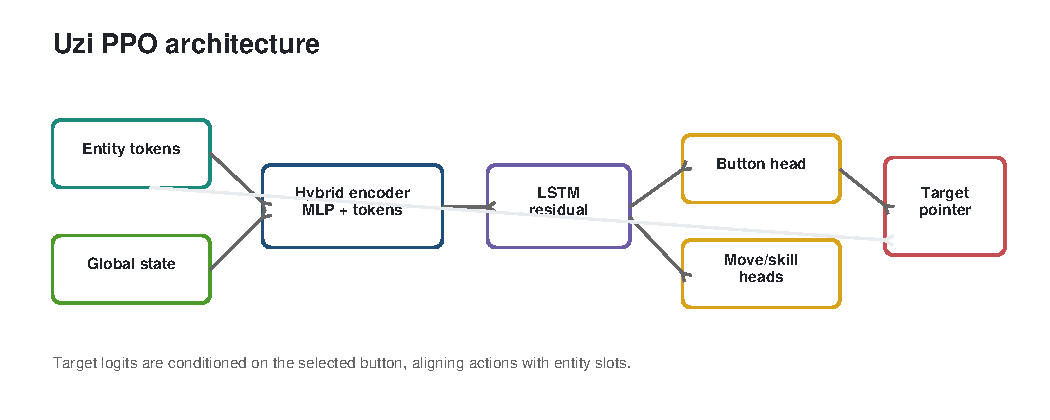
\includegraphics[width=0.86\linewidth]{architecture.pdf}
  \caption{The Uzi policy uses structured entity tokens and global state, fuses them with a raw MLP pathway, applies an LSTM residual, and predicts multi-discrete actions. The target logits are conditioned on the selected top-level button, so target slots are interpreted in the same context as the chosen action.}
  \label{fig:architecture}
\end{figure}

\section{Environment and action interface}

We train in the Honor of Kings 1v1 lane environment with three heroes in the curriculum: Luban No. 7 (112), Di Renjie (133), and Gongsun Li (199). The action label has six components:
\[
  a_t = (b_t, m^x_t, m^z_t, s^x_t, s^z_t, g_t),
\]
where $b_t$ is the button, the middle four heads parameterize movement or skill direction, and $g_t$ is a target slot among None, enemy hero, self, Soldier1--4, tower, and monster. The legal-action vector has two forms in the codebase: a compressed 85-dimensional form and a raw 184-dimensional form in which target legality can depend on the selected button. This detail was central. For example, normal attack with target None or Self is legal-looking in the independent target head but semantically useless. Later versions therefore apply a button-conditioned action-mask adjustment before sampling.

We evaluate evidence at three levels. First, the course leaderboard is the external result: rank 3, 131/67 over 198 games, or 66.2\% aggregate win rate. Second, platform training logs report monitor metrics for individual PPO runs; the final pulled run, \texttt{ppo-5-1}, reached 96,091 learner steps and 20,485 episodes with latest logged win rate 68.8\%. Third, we use synthetic frame probes across historical commits to diagnose code behavior. These probes are not match evaluations; they are deterministic unit-style tests that answer questions such as whether a historical version suppresses invalid Button3 targets.

\section{Method}

\subsection{Structured observation design}

The final feature vector is 561-dimensional. Its main block is a fixed set of entity tokens:
main hero, enemy hero, own and enemy outer towers, four own minions, four enemy minions, one monster, four bullets, and two cakes. A global block stores scalar context such as retreat or recall state. Each token begins with an \texttt{exists} bit used only for padding. Visibility, alive state, time since seen, hero identity, skill state, attack-target relations, bullets, and selected hero-specific mechanics are ordinary features rather than padding gates.

Two details mattered in practice. First, Soldier1--4 target slots are not arbitrary minion order. Environment probes showed that the correct rule is to select visible alive enemy soldiers, choose the nearest four, and then order the selected set by ascending runtime id. This ordering is shared by feature construction, reward target resolution, and target-pointer slots. Second, Gongsun Li has mark state that appears not only on heroes but also on minions. The probe archive observed mark \texttt{19900} with layers 0--3, so the final minion token includes an Arli mark presence/layer pair. This made the failure diagnosable even though it did not fully solve her.

\subsection{Policy and PPO objective}

Figure~\ref{fig:architecture} summarizes the model. A raw MLP pathway preserves direct access to all feature fields. In parallel, entity tokens are projected by type and processed with small AdaLN-conditioned attention blocks. Register tokens summarize the entity set, and a global MLP summarizes scalar context. The structured state is added as a residual to the raw state. A one-layer LSTM residual then gives the policy short-horizon memory for cooldowns, channeling, target disappearance, and recent movement.

The first five action heads use independent categorical logits. The target head is button-conditioned: the policy forms a query from the public state plus a button embedding, then scores target-slot keys derived from entity tokens. During training, the loss gathers target logits for the selected button, so PPO updates the target distribution in the same conditional space used by sampling.

We use the clipped PPO objective \citep{schulman2017ppo} with a value baseline and entropy regularization:
\[
  \mathcal{L}(\theta) =
  \mathbb{E}_t \left[
  -\min(r_t(\theta) \hat{A}_t,
       \mathrm{clip}(r_t(\theta), 1-\epsilon, 1+\epsilon)\hat{A}_t)
  + c_v (V_\theta(s_t)-R_t)^2
  - c_e H(\pi_\theta(\cdot|s_t))
  \right],
\]
where advantages are computed in the platform workflow using generalized-advantage style returns \citep{schulman2015gae}. In our setting the most important implementation point was not the equation itself, but ensuring that the legal mask, old action probabilities, and conditional target logits described the same action.

\subsection{Reward shaping and curriculum}

The reward is target-first. It combines zero-sum differences in tower HP, hero HP trades, kills, money, and experience with non-zero-sum action and lane terms: lane progress, lane presence, retreat recovery, last-hit events, last-hit focus, tower-attack action reward, low-health danger penalty, out-of-range attack penalty, invalid normal-attack penalty, no-op opportunity penalty, idle penalty, and terminal win quality. We intentionally keep action-level shaping small. It should break ties and remove pathological behavior, not dominate tower and kill objectives.

The training workflow cycles heroes 112, 133, and 199 across both camps and dynamically mixes self-play with common AI opponents. If the policy is weak against common AI, the workflow shifts more training episodes toward common AI; if it starts winning, it restores more self-play. This curriculum kept the policy from overfitting only to its current self while still letting aggressive lane patterns sharpen through mirror play.

\section{Results}

\begin{figure}[t]
  \centering
  \begin{minipage}{0.39\linewidth}
    \centering
    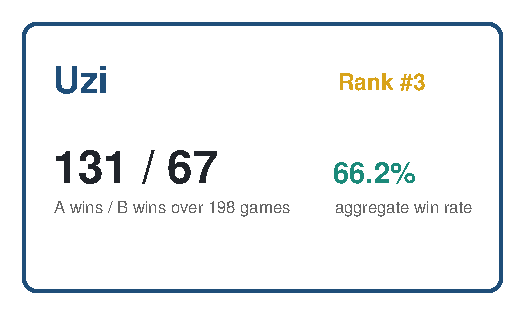
\includegraphics[width=\linewidth]{leaderboard_card.pdf}
  \end{minipage}
  \hfill
  \begin{minipage}{0.57\linewidth}
    \centering
    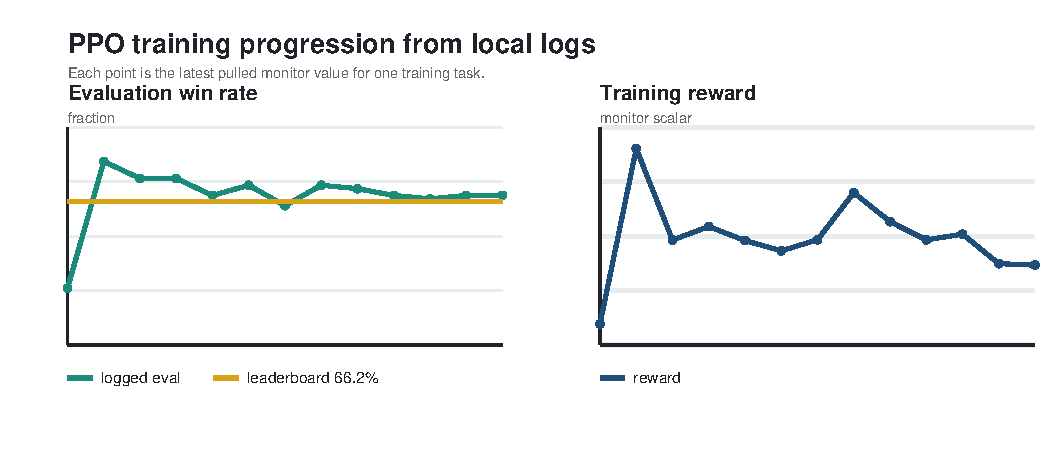
\includegraphics[width=\linewidth]{training_progress.pdf}
  \end{minipage}
  \caption{External and internal performance evidence. The leaderboard result is the main final result: rank 3, 131/67 over 198 games. The training plot shows pulled monitor values across local PPO tasks; \texttt{ppo-5-1} is the final submitted training run in the local logs.}
  \label{fig:performance}
\end{figure}

\begin{table}[t]
  \centering
  \caption{Latest monitor values for the last eight PPO runs. Win rate is the pulled platform monitor value for each training task, not the final leaderboard. Button9 is recall.}
  \label{tab:runs}
  \small
  \begin{tabular}{lrrrrrrr}
    \toprule
    Run & Reward & Win \% & Kill & Death & Self tower & Enemy tower & Button9 \\
    \midrule
    ppo-2-0 & 14.3 & 73.4 & 2.55 & 1.48 & 7689 & 2904 & 0 \\
    ppo-3-1 & 19.1 & 64.1 & 2.95 & 2.14 & 6410 & 3592 & 311 \\
    ppo-4-2 & 39.7 & 73.4 & 3.53 & 1.55 & 7305 & 2470 & 357 \\
    ppo-4-3 & 27.1 & 71.9 & 3.11 & 1.56 & 7634 & 2807 & 335 \\
    ppo-4-4 & 19.0 & 68.8 & 2.52 & 1.11 & 7213 & 3395 & 292 \\
    ppo-4-5 & 21.6 & 67.2 & 2.89 & 0.97 & 7120 & 3735 & 238 \\
    ppo-4-6 & 8.6 & 68.8 & 2.34 & 0.67 & 7562 & 3573 & 216 \\
    ppo-5-1 & 8.0 & 68.8 & 2.30 & 0.92 & 7406 & 3411 & 0 \\
    \bottomrule
  \end{tabular}
\end{table}

Figure~\ref{fig:performance} and Table~\ref{tab:runs} show the two main quantitative views. The leaderboard result is lower than the best single logged monitor run, which is expected because the leaderboard is a broader external evaluation rather than a latest-window training monitor. The final local run, \texttt{ppo-5-1}, reports 68.8\% latest win rate, 2.30 kills, 0.92 deaths, 7406 self tower HP, 3411 enemy tower HP, and zero recall actions in the latest monitor window. The zero Button9 count is intentional: after recall experiments, the final configuration disabled recall and returned to a simpler lane-pressure policy.

\begin{figure}[t]
  \centering
  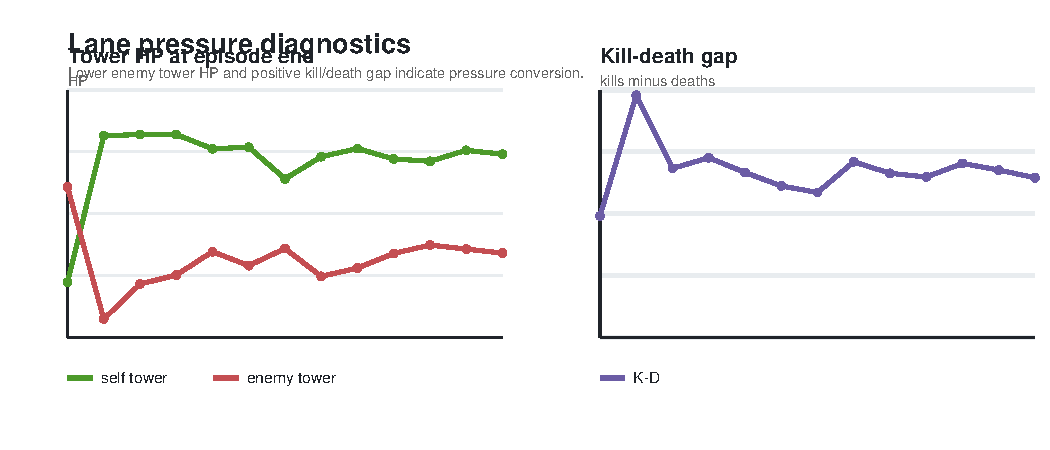
\includegraphics[width=0.82\linewidth]{lane_pressure.pdf}
  \caption{Lane pressure metrics across PPO runs. Uzi's intended style appears in the combination of preserving own tower HP, reducing enemy tower HP, and maintaining a positive kill-death gap.}
  \label{fig:lane-pressure}
\end{figure}

The strongest logged training window was \texttt{ppo-0-11}, with 84.4\% monitor win rate and enemy tower HP near 748. Later runs traded peak monitor reward for multi-hero robustness, recall experiments, and final simplification. This is visible in Figure~\ref{fig:lane-pressure}: tower and kill-death metrics remain positive, but recall-enabled runs introduce noise and lower final HP. This shaped our final story: Uzi should be judged as a strong lane-pressure agent, not as a complete MOBA agent with every macro mechanic.

\section{Case studies}

\subsection{Case study 1: target semantics were a hidden bottleneck}

The first important failure was not reward, but target identity. In a synthetic frame with three enemy minions whose distance order is $[30,20,10]$ but runtime-id order is $[10,20,30]$, early PPO migration commits either lacked the shared target helper or could not expose the relevant mask repair path. From \texttt{f5ce14f} onward, the soldier helper returned $[10,20,30]$, matching the runtime-id slot rule inferred from real diagnostic probes. From \texttt{4c07829} onward, the action-mask helper also suppresses normal attack when its only legal targets are None/Self. This explains why the agent became more reliably aggressive: it stopped spending probability on attacks that could not connect to the intended entity.

\begin{table}[t]
  \centering
  \caption{Historical synthetic probes. ``Mask'' means Button3 is suppressed when only None/Self targets are available. ``Soldier slots'' are returned runtime ids for the constructed frame. Recall is the low-health safe-state reward after enabling recall for probe versions that support it.}
  \label{tab:probes}
  \small
  \begin{tabular}{lrrrr}
    \toprule
    Version & Mask & Soldier slots & Recall & Arli mark \\
    \midrule
    training\_observability\_masks & yes & 10,20,30 & 0.000 & yes \\
    multi\_hero\_curriculum & yes & 10,20,30 & 0.000 & yes \\
    recall\_reward\_shaping & yes & 10,20,30 & 0.060 & yes \\
    temporary\_recall\_exploration & yes & 10,20,30 & 0.060 & yes \\
    recall\_button\_legal & yes & 10,20,30 & 0.060 & yes \\
    recall\_ignition\_monitoring & yes & 10,20,30 & 0.060 & yes \\
    recall\_channel\_state & yes & 10,20,30 & 0.060 & yes \\
    \bottomrule
  \end{tabular}
\end{table}

\subsection{Case study 2: recall was engineered, then removed}

Recall is attractive: a low-health hero can return safely and avoid death. It is also a sparse multi-step channel behavior. The code history shows that we tried more than a reward term. Commit \texttt{a824774} added recall recovery shaping. Commit \texttt{19fd508} added bounded training-only recall exploration. Commit \texttt{3463df5} made Button9 legal for exploration. Later commits added staged ignition rewards, monitoring, and channel-state features. The synthetic low-HP safe probe confirms that those versions assign a positive recall-start reward of 0.06 and record \texttt{recall\_need\_cnt=1}.

\begin{figure}[t]
  \centering
  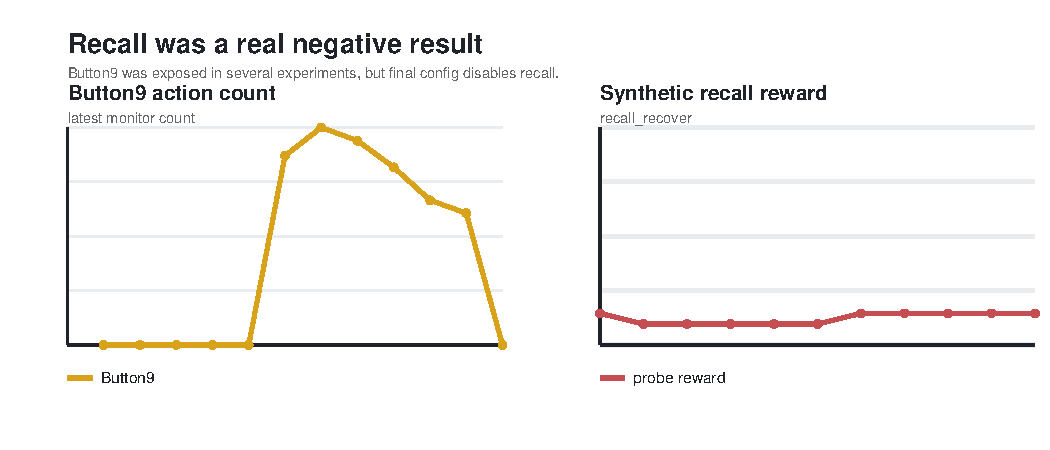
\includegraphics[width=0.82\linewidth]{recall_diagnostics.pdf}
  \caption{Recall experiments. Several historical runs exposed Button9 and produced recall reward in synthetic low-HP safe states, but the final \texttt{ppo-5-1} logs show Button9 count 0. The final system treats recall as a negative result rather than hiding it.}
  \label{fig:recall}
\end{figure}

The problem was that starting recall is not the same as completing recall. A channel can be interrupted by movement, attacks, incoming pressure, or legal-mask changes, and successful healing occurs only after a delayed sequence. In training, this competed with simpler behaviors that were easier to credit: walking back, staying under tower, using lane presence, or continuing to pressure if enemy tower HP was low. The final configuration therefore sets \texttt{RECALL\_ENABLED=False} and reward weight 0.0. This is an honest negative result: we knew how to make the code produce recall incentives, but not how to make the learned policy use recall robustly enough for submission.

\subsection{Case study 3: Gongsun Li remained the hardest hero}

Gongsun Li was the clearest hero-specific failure. The diagnostic archive proves that her mechanics are observable: mark \texttt{19900} appears on minions with multiple layers, and the final feature vector exposes an Arli mark field with nonzero values on real captured frames. However, observability did not imply mastery. Her useful behavior depends on mark timing, displacement, and returning umbrella state, while the shared reward still mostly celebrates generic lane outcomes such as tower damage, safe HP trades, and last hits.

Our interpretation is that the multi-hero policy learned a robust marksman template that fits Luban and Di Renjie better than Gongsun Li. This is consistent with the zero-win-rate failure case: Arli's state variables existed, but the reward and data distribution did not force the policy to use them. A more principled fix would be hero-conditioned reward weights, per-hero heads or adapters, and targeted Arli curriculum episodes rather than assuming one lane-bully objective is equally learnable for all heroes.

\section{Limitations and discussion}

The results should be read with the right evidence boundary. The leaderboard number is the final external result. The training logs are pulled platform monitors from local tasks and are useful for trend analysis, but they are not a controlled ablation suite. The synthetic probes are deterministic diagnostics over code behavior; they explain why a design was plausible, not how many games it wins by itself. Finally, the working tree at the time of writing includes uncommitted PPO changes outside the paper output directory; all probe outputs record whether they came from the dirty working tree or a clean historical worktree.

Despite these limits, the project suggests a concrete recipe for course-scale MOBA RL. First, fix semantics before tuning reward. A policy cannot learn precise aggression if target slots are inconsistent. Second, make action masks reflect game meaning, especially when the action space is factored. Third, keep reward shaping aligned with the desired style: pressure is rewarded, but low-health danger and invalid actions must be punished. Fourth, treat negative results as evidence. The failed recall experiment improved our understanding of temporal credit assignment, and the Arli failure clarified where shared policies stop being enough.

\section{Conclusion}

Uzi ranked third on the course leaderboard with a 66.2\% aggregate result over 198 games. More importantly, the agent's behavior was produced by an interpretable training story: structured entity observations, button-conditioned targets, action-mask repair, lane-pressure rewards, curriculum, and diagnostic probes all pushed in the same direction. We did not train a complete MOBA intelligence. We trained a strong laner, and the most useful engineering lesson is that ``aggressive'' behavior in RL becomes reliable only when the code agrees on what a target, a legal attack, a safe trade, and a won lane actually mean.

\bibliographystyle{plainnat}
\bibliography{references}

\appendix

\section{Data and reproducibility notes}

All generated paper artifacts are under \texttt{outputs/uzi-lane-paper}. The main scripts are:
\begin{itemize}
  \item \texttt{outputs/uzi-lane-paper/probes/run\_historical\_probes.py}: creates temporary detached git worktrees and runs deterministic synthetic frame probes on selected commits.
  \item \texttt{outputs/uzi-lane-paper/data/build\_analysis.py}: parses \texttt{logs/ppo-*}, the final leaderboard record, and historical probe JSON files, then emits CSV tables and vector PDF figures.
\end{itemize}

The final local run summary is \texttt{logs/ppo-5-1/summary.json}. The associated error-log pull reports zero warning/error entries in \texttt{logs/ppo-5-1/errors.jsonl.summary.json}. The probe archive \texttt{diag\_feature\_probes/FEATURE\_PROBE\_SUMMARY.md} is the primary real-frame evidence for Soldier slot ordering, bullet observability, ability bits, Arli marks, and attack-target relations.

\section{Additional historical probe matrix}

\begin{figure}[H]
  \centering
  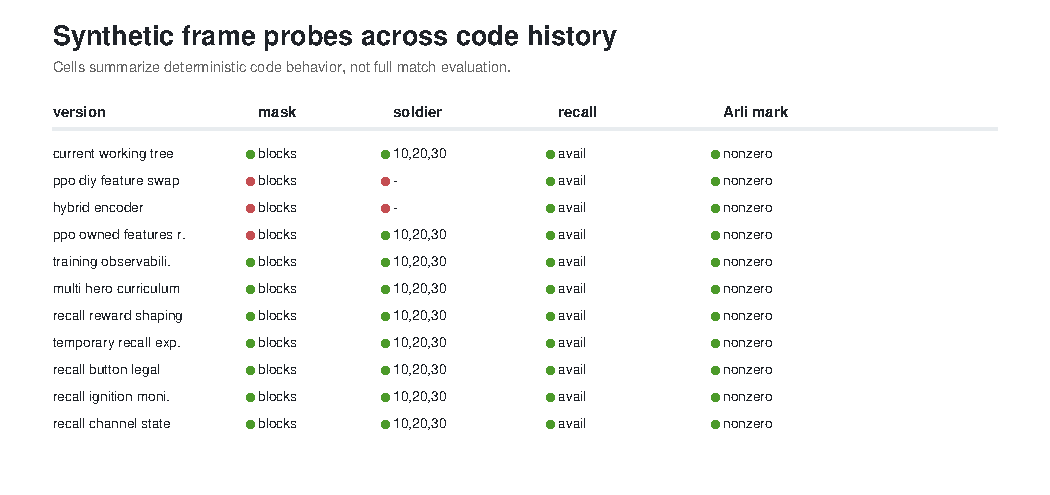
\includegraphics[width=0.92\linewidth]{historical_probe_matrix.pdf}
  \caption{Compact visualization of the synthetic frame probes across selected historical commits.}
  \label{fig:probe-matrix}
\end{figure}

\section{Code package manifest}

The submission code package should include:
\begin{itemize}
  \item \texttt{agent\_ppo/}: final PPO agent implementation.
  \item \texttt{agent\_diy/}: earlier feature/reward implementation used during migration and comparison.
  \item \texttt{script/pull\_training\_data.py}, \texttt{script/diag\_feature\_probe.py}, and related diagnostics.
  \item \texttt{logs/ppo-5-1/}: final training metrics and empty pulled error log.
  \item \texttt{diag\_feature\_probes/}: real environment diagnostic frames.
  \item \texttt{outputs/uzi-lane-paper/}: paper, poster, generated figures, synthetic probe outputs, and analysis CSV files.
\end{itemize}

\end{document}
